\documentclass[resume]{subfiles}


\begin{document}
\section{Fonctions de transfert}
\subsection{Marge de gain / marge de phase}
\begin{figure}[H]
\centering
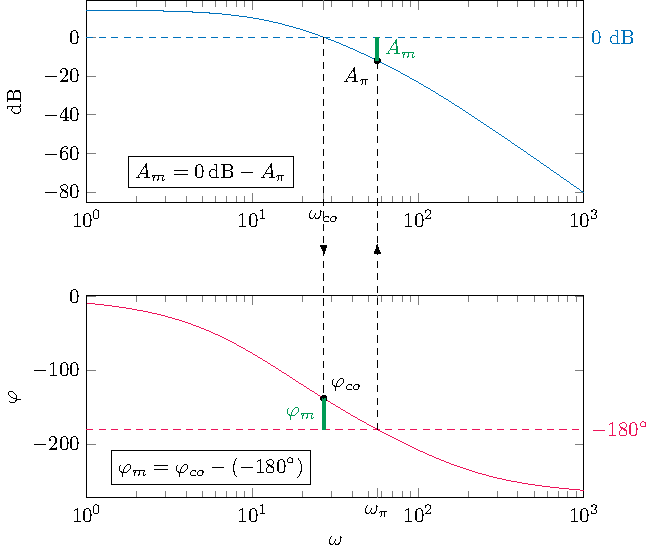
\includegraphics[width=\columnwidth]{drwg_4.pdf}
\end{figure}
\subsection{Équations aux différences}
\label{sec_eq_diff}
$$\LARGE \underset{\text{degré relatif}}{d}=\underset{\deg(\text{denominateur})}{n}-\underset{\deg(\text{numérateur})}{m}$$
Forme développée ($Y$ en fonction de $U$)
\begin{multline*}
Y(z)\left(\textcolor{Gray}{a_0=1}+\acolor{a_1}z^{-1}+\acolor{a_2}z^{-2}+\cdots+\acolor{a_n}z^{-n}\right)=\\U(z)\left(\bcolor{b_0}z^{-d}+\bcolor{b_1}z^{-d-1}+\bcolor{b_2}z^{-d-2}+\cdots+\bcolor{b_m}z^{-d-m}\right)
\end{multline*}
Forme fonction de transfert avec puissances de $z$ négatives
On peut aussi écrire sous la forme $z^{-x}$
$$G(z)=\frac{\bcolor{b_0}z^{-d}+\bcolor{b_1}z^{-d-1}+\bcolor{b_2}z^{-d-2}+\cdots+\bcolor{b_m}z^{-d-m}}{\textcolor{Gray}{a_0}+\acolor{a_1}z^{-1}+\acolor{a_2}z^{-2}+\cdots+\acolor{a_n}z^{-n}}$$
$$G(z)=\frac{Y(z)}{U(z)}$$
\end{document}